% Versão didática e pareada do relatório da execução de produção de 29/10/2026 (DATA_PRP_20C).
% Só entram as tarefas que podem ser pareadas entre os três métodos.
% Tabelas e figuras: docs/gap-analysis/production-run-20261029/pareado/generate_report.py
%   (gera generated/*.tex e figures/production-run-pareado-*.pdf).

\documentclass[11pt,a4paper]{article}

\usepackage[T1]{fontenc}
\usepackage[utf8]{inputenc}
\usepackage[brazil]{babel}
\usepackage{amsmath,amssymb}
\usepackage{booktabs}
\usepackage{geometry}
\usepackage{hyperref}
\usepackage{enumitem}
\usepackage{graphicx}
\usepackage{float}

\geometry{margin=2.5cm}
\hypersetup{colorlinks=true,linkcolor=blue,urlcolor=blue}
\setlength{\parskip}{0.4em}

\newcommand{\nTasks}{900}
\newcommand{\nPaired}{446}
\newcommand{\nExcluded}{454}
\newcommand{\sdFOA}{0,0563}
\newcommand{\meanFOA}{0,2650}
\newcommand{\cvFOA}{21\%}
\newcommand{\minFOA}{0,1653}
\newcommand{\maxFOA}{0,4832}
\newcommand{\sdDiffAC}{12,0\%}
\newcommand{\sePaired}{0,6}
\newcommand{\seUnpaired}{1,4}

\newcommand{\boundDiffMedian}{0,00\%}
\newcommand{\boundDiffMean}{-0,02\%}

\newcommand{\gainMedian}{5,6\%}
\newcommand{\gainMax}{43\%}


\newcommand{\FO}{\mathrm{FO}}

\title{Execução de Produção de 29/10/2026\\
       Impacto dos Métodos e Desempenho do Gap\\
       \large Comparação pareada, explicada passo a passo}
\author{Implementação do repositório LSVRP}
\date{\today}

\begin{document}

\maketitle

\begin{abstract}
\sloppy
Este documento compara três métodos para obter a solução de um problema
multiobjetivo de produção e roteamento, a partir da execução de produção no
cluster: uma heurística de enxame de partículas seguida do MIP, uma
matheurística seguida do MIP e a matheurística sozinha. A comparação é
\emph{pareada}: só entram as \nPaired{} tarefas em que os três métodos
produziram resultados comparáveis. A análise tem duas frentes: (i) quanto o
método muda a qualidade da solução e (ii) como se comporta o \emph{gap}, a medida
de distância ao ótimo. A cada tabela e a cada figura explicamos o que ela mostra
e como interpretá-la. Nas tarefas analisadas os três métodos são praticamente
equivalentes na qualidade da solução (diferenças de até cerca de 0,4\% na média,
dentro da incerteza), o limite inferior do MIP é o mesmo nos dois métodos que o
usam, e o gap mediano é de cerca de 11\%, variando muito com o vetor de pesos.
\end{abstract}

\section*{Como ler este documento}

Estes termos aparecem em todo o texto:

\begin{description}[leftmargin=1.5em,style=nextline]
  \item[Tarefa] Uma combinação de uma instância (um dos 150 arquivos de 20
  clientes) com um vetor de pesos (6 vetores). Cada método resolve as mesmas
  tarefas, o que permite comparar os métodos tarefa a tarefa.
  \item[FO (função objetivo)] O valor que o otimizador tenta minimizar:
  \emph{quanto menor, melhor}. O vetor de pesos muda o que a FO mede; por isso
  só se comparam valores de FO de métodos diferentes \emph{na mesma tarefa} (ou
  médias sobre as mesmas tarefas).
  \item[Incumbente] A melhor solução viável encontrada até o fim do tempo.
  \item[Limite inferior] Um valor abaixo do qual o MIP prova que nenhuma solução
  pode ficar. O ótimo verdadeiro está entre o limite inferior e a incumbente.
  \item[Gap] A distância relativa entre a incumbente e o limite inferior:
  \[
    \text{gap} = \frac{\text{incumbente} - \text{limite inferior}}{\text{incumbente}}.
  \]
  Um gap de 10\% garante que a solução está, no máximo, 10\% acima do melhor
  valor possível. Gap menor é melhor; gap 0 significa ótimo provado. É a
  medida de otimalidade usada na pesquisa.
\end{description}

Os três métodos comparados (todos com 1 thread, orçamento total de 3600~s por
tarefa e o modelo sem índice de veículo):

\begin{itemize}[leftmargin=*]
  \item \textbf{A, PSO + MIP}: uma heurística de enxame de partículas (PSO) gera
  uma solução inicial, e o MIP completo (CPLEX) parte dela. A partir de 3000~s
  de tarefa o CPLEX passa a usar \emph{solution polishing} (uma busca focada em
  melhorar a incumbente).
  \item \textbf{B, matheurística + MIP}: uma matheurística (primeiro fixa a ordem
  das visitas por um TSP, depois resolve um MIP restrito a essa ordem, a partir
  de uma solução do PSO) gera a solução inicial, e o MIP completo parte dela,
  também com polishing após 3000~s.
  \item \textbf{C, matheurística}: só a matheurística, com o estágio restrito
  usando o orçamento inteiro, sem MIP completo. Por isso o método C não tem gap.
\end{itemize}

\section{As tarefas analisadas}

\begin{table}[H]
  \centering
  \small
  \begin{tabular}{lrr}
\toprule
Método & Tarefas com resultado & Tarefas analisadas (pareadas) \\
\midrule
A. PSO + MIP & 900 & 446 \\
B. Matheurística + MIP & 900 & 446 \\
C. Matheurística & 894 & 446 \\
\bottomrule
\end{tabular}

  \caption{Tarefas com resultado e tarefas analisadas em cada método.}
  \label{tab:execucao}
\end{table}

\paragraph{O que a tabela mostra.} Cada método foi executado sobre as mesmas
\nTasks{} tarefas. A segunda coluna é o número de tarefas com algum resultado
(o método C ficou com 894); a terceira é o número de tarefas usadas neste
documento.

\paragraph{Como as tarefas foram escolhidas.} Para comparar métodos de forma
justa, usamos só as \nPaired{} tarefas em que os três métodos produziram
resultados \emph{pareáveis}: o MIP foi aceito na validação do projeto tanto no
método A quanto no B (de modo que as soluções e os gaps são do MIP e não da
heurística), e a tarefa existe também no método C. As demais \nExcluded{} tarefas
não podem ser pareadas e foram descartadas.

\paragraph{Cuidado ao interpretar.} Essa escolha não é aleatória: as tarefas
analisadas são aquelas em que o MIP produziu uma solução aceita pela validação.
O número de tarefas por vetor de pesos varia (de 55 a 99, ver
Tabela~\ref{tab:fo-peso}), então os resultados valem para este conjunto e não
necessariamente para todas as 900 tarefas. A causa do descarte do MIP nas
demais tarefas está sendo investigada à parte.

\section{Frente (i): impacto dos métodos na solução}

\subsection{Como a função objetivo se distribui}

\begin{table}[H]
  \centering
  \small
  \begin{tabular}{lrrrrrr}
\toprule
Método & n & Média & Mediana & P10 & P90 & Máx. \\
\midrule
A. PSO + MIP & 446 & 0,2650 & 0,2525 & 0,2024 & 0,3469 & 0,4832 \\
B. Matheurística + MIP & 446 & 0,2666 & 0,2526 & 0,2062 & 0,3484 & 0,4945 \\
C. Matheurística & 446 & 0,2676 & 0,2534 & 0,2043 & 0,3476 & 0,4926 \\
\bottomrule
\end{tabular}

  \caption{FO por método nas \nPaired{} tarefas analisadas (menor é melhor).}
  \label{tab:fo-dist}
\end{table}

\paragraph{O que a tabela mostra.} Cada linha resume os \emph{n} valores de FO de
um método: a média, a mediana (o valor que divide as tarefas ao meio), o P10 (10\%
das tarefas têm FO abaixo dele), o P90 (10\% têm FO acima dele) e o máximo.

\paragraph{Como interpretar.} As três linhas são muito parecidas: médias entre
0,2650 e 0,2676 (diferença de cerca de 1\%) e medianas praticamente iguais (0,2525 a
0,2534). Ao mesmo tempo a FO varia bastante \emph{entre tarefas}: no método A o desvio
padrão é \sdFOA{} para uma média de \meanFOA{} (cerca de \cvFOA{} da média), com mínimo \minFOA{} e
máximo \maxFOA{}. Diferenças entre os métodos de poucos décimos de ponto percentual são
pequenas diante dessa variação natural, o que motiva a comparação pareada da seção
seguinte.

\subsection{Comparação pareada}

\subsubsection*{Por que comparar tarefa a tarefa}

Comparar apenas as médias da Tabela~\ref{tab:fo-dist} mistura dois efeitos: a
diferença entre os métodos e a diferença entre as tarefas (instâncias mais difíceis
têm FO maior para qualquer método). Como cada método resolveu as \emph{mesmas}
tarefas, podemos comparar dois métodos \emph{dentro de cada tarefa}, o que remove
a variação entre tarefas. A isso se chama comparação pareada. Para cada tarefa
calculamos
\[
  d = \frac{\FO_{1} - \FO_{2}}{\FO_{2}},
\]
a diferença relativa do primeiro método em relação ao segundo. Se $d$ é
\emph{negativo}, o primeiro método é melhor naquela tarefa; se é positivo, é
pior; $d = 0{,}01$ significa 1\% pior.

\paragraph{Exemplo.} Na tarefa \texttt{PRP13\_C20\_P8\_V5\_T12\_S2} com pesos (0,3; 0,3; 0,1; 0,2; 0,1) os três métodos obtiveram:

\begin{table}[H]
  \centering
  \small
  \begin{tabular}{lrr}
\toprule
Método & FO da tarefa & Diferença em relação a C \\
\midrule
A. PSO + MIP & 0,2358 & 0,23\% \\
B. Matheurística + MIP & 0,2394 & 1,74\% \\
C. Matheurística & 0,2353 & -- \\
\bottomrule
\end{tabular}

  \caption{Exemplo de uma tarefa. A coluna da direita é $d$ em relação ao método C.}
  \label{tab:exemplo}
\end{table}

Aqui A ficou 0,23\% pior que C e B ficou 1,74\% pior. Repetindo esse cálculo nas
\nPaired{} tarefas obtemos uma distribuição de valores de $d$, que a tabela e a
figura abaixo resumem. O pareamento importa: a FO varia cerca de \cvFOA{} entre tarefas,
enquanto o desvio padrão de $d$ entre A e C é de \sdDiffAC{}. Na ordem de grandeza, com
\nPaired{} tarefas, o erro da média das diferenças é de cerca de \sePaired{} ponto percentual
com o pareamento e cerca de \seUnpaired{} sem ele.

\subsubsection*{Como ler as colunas da tabela pareada}

\begin{description}[leftmargin=1.5em,style=nextline]
  \item[n] Quantas tarefas entram na comparação.
  \item[1º melhor] Fração de tarefas em que o primeiro método teve FO menor ($d<0$).
  \item[Empate] Fração de tarefas com FO igual (diferença menor que $10^{-9}$). Ocorre
  quando os dois métodos terminam com exatamente a mesma solução.
  \item[Mediana] O valor típico de $d$: metade das tarefas tem $d$ menor e metade
  maior. É pouco sensível a casos extremos.
  \item[Média] A média de $d$. É sensível a casos extremos: algumas tarefas muito
  ruins puxam a média para cima. Quando a média é bem maior que a mediana, há uma
  cauda de tarefas em que o primeiro método é muito pior.
  \item[IC 95\% da média] Um intervalo de confiança calculado por \emph{bootstrap}:
  sorteamos 4000 vezes, com reposição, um conjunto de tarefas do mesmo tamanho,
  recalculamos a média de $d$ em cada sorteio e tomamos os percentis 2,5\% e 97,5\%
  das 4000 médias. Ele mostra a incerteza da média por termos olhado só estas
  tarefas.
\end{description}

\paragraph{Regra prática.} Se o intervalo \emph{contém o zero}, a diferença média
pode ser apenas ruído: com estes dados não se distingue um método do outro. Se o
intervalo está inteiro de um lado do zero, a diferença é provavelmente real (e
ainda é preciso julgar se é grande o bastante para importar).

\begin{table}[H]
  \centering
  \scriptsize
  \begin{tabular}{lrrrrrr}
\toprule
Comparação (1º contra 2º) & n & 1º melhor & Empate & Mediana & Média & IC 95\% da média \\
\midrule
A contra B & 446 & 60\% & 0\% & -0,19\% & -0,33\% & [-0,97\%; 0,31\%] \\
A contra C & 446 & 46\% & 0\% & 0,22\% & -0,16\% & [-1,23\%; 1,01\%] \\
B contra C & 446 & 41\% & 2\% & 0,38\% & 0,35\% & [-0,71\%; 1,46\%] \\
\bottomrule
\end{tabular}

  \caption{Comparação pareada da FO nas \nPaired{} tarefas analisadas.}
  \label{tab:pareada}
\end{table}

\paragraph{Como interpretar a Tabela~\ref{tab:pareada}.}
\begin{itemize}[leftmargin=*]
  \item \emph{A contra B} (PSO + MIP contra matheurística + MIP): A é melhor em
  60\% das tarefas, a mediana de $d$ é $-0{,}19\%$ e a média $-0{,}33\%$, com intervalo
  [$-0{,}97\%$; $+0{,}31\%$]. O intervalo contém o zero: os dois métodos com MIP não se
  distinguem, apesar de A ganhar na maior parte das tarefas.
  \item \emph{A contra C} (PSO + MIP contra matheurística): A é melhor em 46\% das
  tarefas, com mediana $+0{,}22\%$ e média $-0{,}16\%$, intervalo [$-1{,}23\%$; $+1{,}01\%$].
  Contém o zero.
  \item \emph{B contra C}: B é melhor em 41\% das tarefas (e há 2\% de empates), com mediana
  $+0{,}38\%$ e média $+0{,}35\%$, intervalo [$-0{,}71\%$; $+1{,}46\%$]. Contém o zero.
\end{itemize}
Em resumo, \emph{nenhuma} diferença entre os métodos é distinguível de zero: nas
tarefas analisadas, adicionar o MIP completo depois da matheurística, ou trocar o
ponto de partida do MIP, não muda a qualidade da solução de modo mensurável. Os
intervalos mostram que, com estes dados, diferenças reais acima de cerca de 1\% a 1,5\%
já seriam detectadas.

\begin{figure}[H]
  \centering
  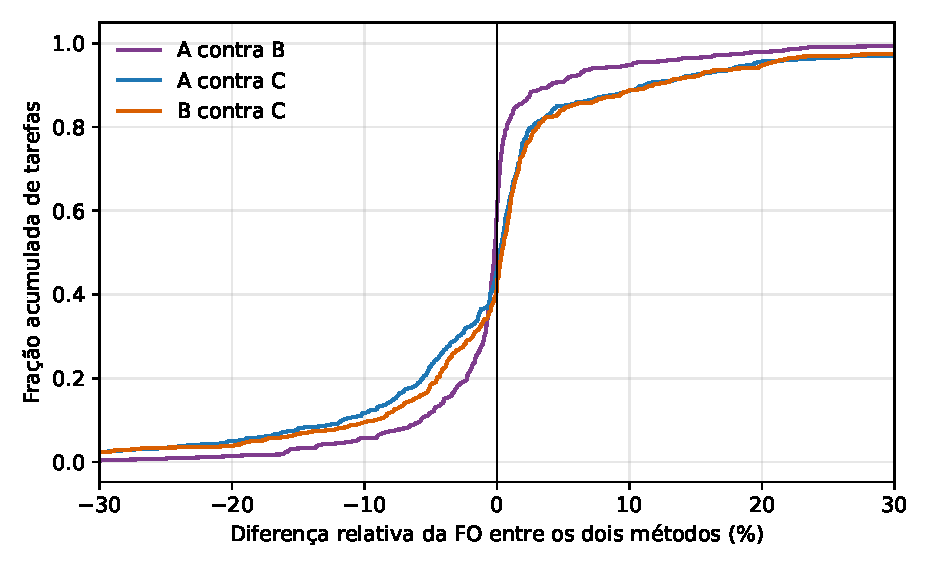
\includegraphics[width=0.8\textwidth]{figures/production-run-pareado-fo-diff-cdf.pdf}
  \caption{Distribuição acumulada da diferença relativa da FO entre pares de
  métodos, nas \nPaired{} tarefas analisadas.}
  \label{fig:fo-diff}
\end{figure}

\subsubsection*{Como ler a Figura~\ref{fig:fo-diff}}

A figura mostra a distribuição inteira de $d$, não só a média. Cada curva é uma
comparação (por exemplo, ``A contra C'' usa $d=(\FO_A-\FO_C)/\FO_C$). O eixo
horizontal é $d$ em pontos percentuais; o eixo vertical é a fração acumulada: o
ponto $(x,y)$ de uma curva diz que $y$ das tarefas têm $d \le x$. A linha vertical
preta marca $d=0$: \emph{à esquerda}, o primeiro método é melhor; \emph{à direita},
é pior.

\begin{itemize}[leftmargin=*]
  \item \textbf{Onde a curva cruza o zero} é a fração de tarefas em que o primeiro
  método é melhor ou igual ao segundo (Tabela~\ref{tab:fig-leitura}, coluna $x\le 0$).
  \item \textbf{A subida íngreme perto de zero} mostra que na maioria das tarefas a diferença
  entre os métodos é pequena.
  \item \textbf{As caudas} (as pontas esquerda e direita, em que a curva se aproxima lentamente
  de 0 e de 1) mostram as tarefas em que um método é bem melhor ou bem pior que o outro.
  \item \textbf{Curvas que se sobrepõem} indicam métodos com o mesmo perfil de desempenho.
\end{itemize}

\begin{table}[H]
  \centering
  \small
  \begin{tabular}{lrrrr}
\toprule
Curva & $x\le -5\%$ & $x\le 0$ (melhor ou igual) & $x\le +5\%$ & $x\le +10\%$ \\
\midrule
A contra B & 12\% & 60\% & 91\% & 95\% \\
A contra C & 23\% & 46\% & 85\% & 89\% \\
B contra C & 18\% & 43\% & 84\% & 89\% \\
\bottomrule
\end{tabular}

  \caption{Leitura numérica das curvas da Figura~\ref{fig:fo-diff} em $x=-5\%$, $0$, $+5\%$ e
  $+10\%$ (fração acumulada de tarefas). A coluna $x\le 0$ inclui empates.}
  \label{tab:fig-leitura}
\end{table}

\paragraph{O que a figura mostra.} As três curvas cruzam o zero em 60\% (A contra B),
46\% (A contra C) e 43\% (B contra C), e sobem rápido perto de zero: a diferença fica
entre $-5\%$ e $+5\%$ em 79\% das tarefas na comparação A contra B, 62\% em A contra C e
66\% em B contra C. As caudas são curtas e simétricas: em A contra C, 23\% das tarefas
têm A mais de 5\% melhor que C e 15\% têm A mais de 5\% pior. Isso confirma o que a
Tabela~\ref{tab:pareada} mostrou: os métodos se equivalem em média, com tarefas em que
um ou outro ganha por alguns pontos percentuais.

\subsection{Por vetor de pesos e por classe de instância}

\begin{table}[H]
  \centering
  \small
  \begin{tabular}{lrrrr}
\toprule
Pesos $w_1,\ldots,w_5$ & n & A & B & C \\
\midrule
(0,2; 0,2; 0,2; 0,2; 0,2) & 99 & 0,2579 & 0,2618 & 0,2640 \\
(0,2; 0,5; 0,1; 0,1; 0,1) & 63 & 0,3544 & 0,3551 & 0,3507 \\
(0,25; 0,25; 0,25; 0,125; 0,125) & 67 & 0,2172 & 0,2192 & 0,2350 \\
(0,3; 0,3; 0,1; 0,1; 0,2) & 81 & 0,2682 & 0,2706 & 0,2701 \\
(0,3; 0,3; 0,1; 0,2; 0,1) & 81 & 0,2428 & 0,2426 & 0,2366 \\
(0,35; 0,35; 0,1; 0,1; 0,1) & 55 & 0,2619 & 0,2610 & 0,2609 \\
\bottomrule
\end{tabular}

  \caption{FO média por vetor de pesos e por método, nas tarefas analisadas.}
  \label{tab:fo-peso}
\end{table}

\paragraph{O que a tabela mostra.} Cada linha é um vetor de pesos $(w_1;\ldots;w_5)$,
que dá o peso de cada custo (produção, setup, estoque, transporte fixo e
transporte variável) na FO; ``n'' é o número de tarefas analisadas com aquele vetor.
As colunas A, B e C são a FO média de cada método.

\paragraph{Como interpretar.} Só se comparam números \emph{da mesma linha}: o vetor de
pesos muda a escala da FO (a linha $(0{,}2;0{,}5;\ldots)$ tem FO bem maior que as
demais). Dentro de uma linha, as diferenças são pequenas na maior parte dos vetores. A
exceção é $(0{,}25;0{,}25;0{,}25;0{,}125;0{,}125)$, em que A e B (0,2172 e 0,2192) ficam
cerca de 7\% a 8\% abaixo de C (0,2350). Como são só 67 tarefas nesse vetor e a
comparação pareada geral não mostra diferença, vale tratar esse resultado como um ponto
a confirmar, não como um efeito estabelecido.

\begin{table}[H]
  \centering
  \small
  \begin{tabular}{lrrrr}
\toprule
Classe & n & A & B & C \\
\midrule
1 & 172 & 0,2620 & 0,2647 & 0,2634 \\
2 & 146 & 0,2702 & 0,2723 & 0,2752 \\
3 & 128 & 0,2633 & 0,2627 & 0,2647 \\
\bottomrule
\end{tabular}

  \caption{FO média por classe de instância e por método, nas tarefas analisadas.}
  \label{tab:fo-classe}
\end{table}

\paragraph{O que a tabela mostra e como interpretar.} É o mesmo resumo, agrupado pela
classe da instância (1, 2 ou 3, conforme a coluna \texttt{classe} dos resultados). A classe
2 tem a maior FO média nos três métodos, isto é, tende a ser a de maior custo. Dentro de
cada classe a diferença entre métodos é pequena (no máximo cerca de 1,8\%).

\subsection{Composição da solução}

\begin{table}[H]
  \centering
  \small
  \begin{tabular}{lrrr}
\toprule
Componente (média por tarefa) & A & B contra A & C contra A \\
\midrule
f1 (produção) & 19 073 660 & -0,0\% & 0,0\% \\
f2 (setup) & 18 484 & 0,4\% & 4,1\% \\
f3 (estoque) & 787 164 & -0,3\% & 5,0\% \\
f4 (transp. fixo) & 1 507 753 & 0,1\% & -3,8\% \\
f5 (transp. variável) & 97 070 & 1,8\% & -3,7\% \\
nº de setups (soma de $y$) & 427,9 & 0,2\% & 2,7\% \\
\bottomrule
\end{tabular}

  \caption{Média dos totais de cada componente de custo nas tarefas analisadas.}
  \label{tab:componentes}
\end{table}

\paragraph{O que a tabela mostra.} A FO combina cinco custos: f1 (produção), f2
(setup), f3 (estoque), f4 (transporte fixo, por rota) e f5 (transporte
variável, por distância). A coluna A é a média, por tarefa, do total de cada
custo no horizonte; as colunas ``B contra A'' e ``C contra A'' são a variação
percentual em relação a A. Positivo significa que o método gasta mais naquele
custo que A.

\paragraph{Como interpretar.} A e B têm soluções de composição muito parecida (até 2\%
de diferença). A matheurística (C) troca transporte por setup e estoque:
cerca de 4\% menos transporte (f4 e f5) em troca de 4\% a 5\% mais setup e
estoque (f2 e f3), e 2,7\% mais setups. O custo de produção (f1) é igual nos
três, pois é o mínimo dado pela demanda. Em termos de FO esses ajustes se
compensam, e por isso a FO total não muda.

\subsection{Quanto o MIP melhora a matheurística}

\begin{table}[H]
  \centering
  \small
  \begin{tabular}{rrrrrrr}
\toprule
n & Média & IC 95\% da média & P10 & Mediana & P90 & Máx. \\
\midrule
446 & 9,7\% & [8,9\%; 10,6\%] & 0,6\% & 5,6\% & 25,6\% & 43,2\% \\
\bottomrule
\end{tabular}

  \caption{Melhora relativa da FO do MIP sobre a solução do estágio restrito da
  matheurística (método B), por tarefa.}
  \label{tab:ganho-mip}
\end{table}

\paragraph{O que a tabela mostra.} No método B o MIP parte da solução do estágio
restrito da matheurística (que usa 180~s). A melhora é
$(\FO_{\text{restrito}}-\FO_{\text{MIP}})/\FO_{\text{restrito}}$: positivo significa que o MIP achou
uma solução melhor. A linha resume as \nPaired{} tarefas (média, o intervalo de confiança da
média por \emph{bootstrap}, P10, mediana, P90 e máximo).

\paragraph{Como interpretar.} O MIP melhora a solução inicial em média 9,7\% (intervalo
[8,9\%; 10,6\%], bem longe de zero), com mediana de \gainMedian{} e cauda de até \gainMax{}: o
MIP completo agrega muito sobre o estágio restrito de 180~s. Mesmo assim, a matheurística
sozinha com 3600~s no estágio restrito (método C) fica a 0,4\% de B
(Tabela~\ref{tab:pareada}), sem diferença distinguível: dar mais tempo ao estágio
restrito rende aproximadamente o mesmo que passar ao MIP completo. A comparação mistura
tempo e método, então não separa os dois efeitos.

\section{Frente (ii): desempenho do gap}

O gap (definido no início) só existe nos métodos com MIP; o método C não tem gap por
construção. As análises abaixo usam as mesmas \nPaired{} tarefas, em que o gap de A e o
de B são ambos do MIP.

\begin{table}[H]
  \centering
  \scriptsize
  \resizebox{\textwidth}{!}{\begin{tabular}{lrrrrrrrrr}
\toprule
Método & n & Média & Mediana & P90 & Máx. & $\le 5\%$ & $\le 10\%$ & $\le 20\%$ & Gap $0$ \\
\midrule
A. PSO + MIP & 446 & 16,5\% & 11,6\% & 36,3\% & 54,6\% & 19\% & 46\% & 66\% & 1 \\
B. Matheurística + MIP & 446 & 16,9\% & 11,3\% & 36,7\% & 54,6\% & 19\% & 46\% & 64\% & 2 \\
\bottomrule
\end{tabular}
}
  \caption{Distribuição do gap nas tarefas analisadas.}
  \label{tab:gap-dist}
\end{table}

\paragraph{O que a tabela mostra.} Cada linha é um método. ``n'' é o número de tarefas.
Seguem a média, a mediana, o P90 (90\% das tarefas têm gap abaixo dele) e o máximo.
As colunas ``$\le x\%$'' dão a fração de tarefas com gap menor ou igual a $x$ (por exemplo,
$\le 10\%$ é a fração de tarefas com solução a no máximo 10\% do ótimo). ``Gap 0'' é o número
de tarefas com otimalidade provada.

\paragraph{Como interpretar.} O gap mediano é de cerca de 11\% e a média de 16,5\% a 16,9\%:
a média é maior porque há tarefas com gap muito alto (máximo de 54,6\%). Em 46\% das
tarefas o gap é de até 10\% e em 64\% a 66\% até 20\%. Apenas 1 a 2 tarefas têm ótimo
provado. As duas linhas são praticamente iguais.

\begin{figure}[H]
  \centering
  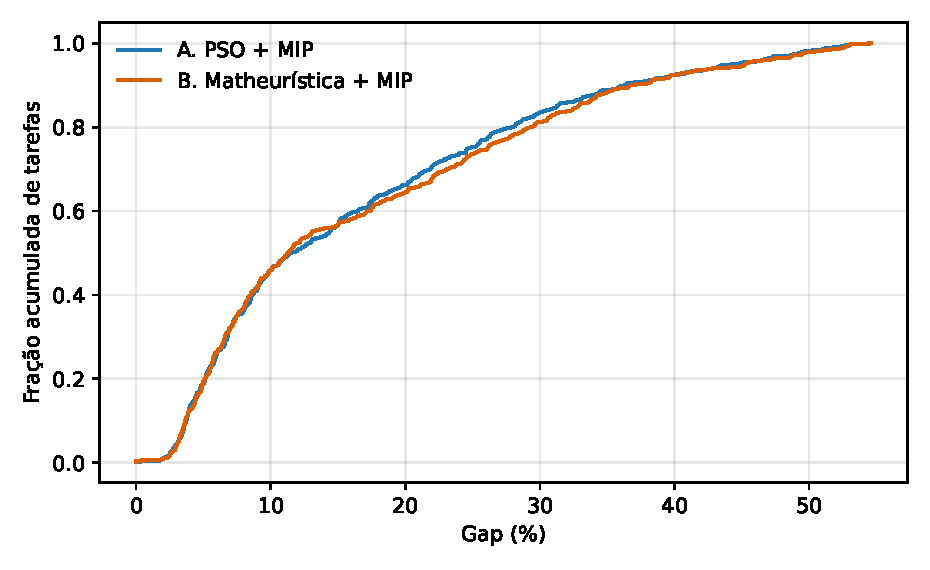
\includegraphics[width=0.8\textwidth]{figures/production-run-pareado-gap-cdf.pdf}
  \caption{Distribuição acumulada do gap nas tarefas analisadas.}
  \label{fig:gap-cdf}
\end{figure}

\subsubsection*{Como ler a Figura~\ref{fig:gap-cdf}}

O eixo horizontal é o gap em \%; o vertical é a fração acumulada de tarefas: o
ponto $(x,y)$ de uma curva diz que $y$ das tarefas têm gap $\le x$. Cada curva é
um método.

\begin{itemize}[leftmargin=*]
  \item \textbf{Quanto mais alta e à esquerda a curva, melhor}: mais tarefas com gap pequeno.
  \item Para ler uma meta, vá ao valor de $x$ e suba até a curva. Em $x=10\%$ as curvas estão em
  cerca de 0,46: 46\% das tarefas têm gap até 10\%. Em $x=20\%$, entre 0,64 e 0,66.
  \item \textbf{O início da curva} (perto de zero) mostra as poucas tarefas com gap quase nulo.
  \item \textbf{A parte final lenta} (curva que demora a chegar a 1) mostra as tarefas em que o MIP
  não conseguiu fechar o gap.
\end{itemize}

\paragraph{O que a figura mostra.} As curvas de A e de B são quase idênticas: os dois
métodos têm a mesma distribuição de gap. O formato é o de uma distribuição assimétrica:
muitas tarefas com gap pequeno ou moderado e uma cauda longa de tarefas difíceis, com
gap de até 55\%.

\subsection{Comparação pareada do gap}

\begin{table}[H]
  \centering
  \scriptsize
  \resizebox{\textwidth}{!}{\begin{tabular}{lrrrrrr}
\toprule
Comparação & n & A menor & Empate & Mediana (p.p.) & Média (p.p.) & IC 95\% da média (p.p.) \\
\midrule
gap de A contra gap de B & 446 & 61\% & 0\% & -0,18 & -0,37 & [-0,90; 0,16] \\
\bottomrule
\end{tabular}
}
  \caption{Diferença do gap entre A e B, tarefa a tarefa, em pontos percentuais (p.p.).}
  \label{tab:gap-pareado}
\end{table}

\paragraph{O que a tabela mostra.} Para cada tarefa, a diferença entre o gap de A e o
gap de B, em pontos percentuais (gap de A menos gap de B). Negativo significa que A tem o
gap menor. As colunas têm o mesmo sentido das tabelas pareadas da FO.

\paragraph{Como interpretar.} A tem o gap menor em 61\% das tarefas, mas a diferença típica
é de $-0{,}18$ ponto percentual e a média de $-0{,}37$, com intervalo [$-0{,}90$; $+0{,}16$] que
contém o zero. Os dois métodos com MIP têm, portanto, o mesmo desempenho de gap.

\subsection{O limite inferior não depende do ponto de partida}

\begin{table}[H]
  \centering
  \small
  \begin{tabular}{lrrr}
\toprule
Método & Limite inferior médio & Incumbente média & Gap médio \\
\midrule
A. PSO + MIP & 0,2205 & 0,2650 & 16,5\% \\
B. Matheurística + MIP & 0,2206 & 0,2666 & 16,9\% \\
\bottomrule
\end{tabular}

  \caption{Limite inferior, incumbente e gap médios. O limite de A é derivado do gap
  reportado (incumbente $\times(1-\text{gap})$).}
  \label{tab:bound}
\end{table}

\paragraph{O que a tabela mostra.} Para cada método, a média do limite inferior, a
média da incumbente e o gap médio. Lembre que gap $=1-\text{limite}/\text{incumbente}$.

\paragraph{Como interpretar.} O limite inferior médio é o mesmo em A e em B (0,2205 contra
0,2206; a diferença mediana por tarefa é \boundDiffMedian{}). Logo, a diferença de gap
entre os dois métodos, quando existe, vem só da incumbente. O limite é fixado pelo
trabalho do CPLEX na raiz (cortes) e não pela solução inicial. Na prática, para reduzir o
gap é preciso ou melhorar a incumbente ou melhorar a formulação (para elevar o limite).

\subsection{Por vetor de pesos e por classe}

\begin{table}[H]
  \centering
  \scriptsize
  \resizebox{\textwidth}{!}{\begin{tabular}{lrrrrr}
\toprule
Pesos $w_1,\ldots,w_5$ & n & A (média) & B (média) & A (mediana) & B (mediana) \\
\midrule
(0,2; 0,2; 0,2; 0,2; 0,2) & 99 & 28,4\% & 29,5\% & 28,5\% & 32,4\% \\
(0,2; 0,5; 0,1; 0,1; 0,1) & 63 & 6,5\% & 6,7\% & 3,8\% & 4,4\% \\
(0,25; 0,25; 0,25; 0,125; 0,125) & 67 & 16,6\% & 17,0\% & 14,1\% & 13,0\% \\
(0,3; 0,3; 0,1; 0,1; 0,2) & 81 & 21,5\% & 21,9\% & 22,5\% & 24,2\% \\
(0,3; 0,3; 0,1; 0,2; 0,1) & 81 & 10,2\% & 10,1\% & 7,9\% & 7,5\% \\
(0,35; 0,35; 0,1; 0,1; 0,1) & 55 & 8,6\% & 8,4\% & 5,8\% & 5,7\% \\
\bottomrule
\end{tabular}
}
  \caption{Gap por vetor de pesos, nas tarefas analisadas.}
  \label{tab:gap-peso}
\end{table}

\paragraph{O que a tabela mostra.} Cada linha é um vetor de pesos e ``n'' o número de
tarefas analisadas com ele. As demais colunas são o gap médio e mediano de A e de B.

\paragraph{Como interpretar.} O vetor de pesos é o que mais explica a variação do gap. Com
pesos iguais o gap médio é de cerca de 28\% a 30\%; com mais peso em f2 ou em f1 e f2
($0{,}2;0{,}5;\ldots$ e $0{,}35;0{,}35;\ldots$) ele cai para 6\% a 9\%. Ainda não investigamos a
causa. Uma hipótese, não testada, é que o peso maior em custos fixos aumenta a parte do
objetivo que o limite já enxerga bem. A e B se comportam da mesma forma em todos os vetores.

\begin{table}[H]
  \centering
  \scriptsize
  \resizebox{\textwidth}{!}{\begin{tabular}{lrrrrr}
\toprule
Classe & n & A (média) & B (média) & A (mediana) & B (mediana) \\
\midrule
1 & 172 & 15,6\% & 16,6\% & 10,1\% & 11,5\% \\
2 & 146 & 18,4\% & 18,7\% & 14,5\% & 15,6\% \\
3 & 128 & 15,6\% & 15,3\% & 12,3\% & 10,0\% \\
\bottomrule
\end{tabular}
}
  \caption{Gap por classe de instância, nas tarefas analisadas.}
  \label{tab:gap-classe}
\end{table}

\paragraph{O que a tabela mostra e como interpretar.} As mesmas colunas, agrupadas pela
classe da instância. O gap médio varia pouco entre as classes (15\% a 19\%), e A e B se
equivalem: a classe da instância importa bem menos que o vetor de pesos.

\subsection{O que o gap mede: um cuidado}

As metas (\emph{targets}) usadas no objetivo vêm de otimizações de cada custo
isolado. Hoje a soma das metas de f1 fica abaixo do custo mínimo de produção em
100\% das instâncias de 20 e de 30 clientes, o que obriga o desvio de f1 a ser positivo em
qualquer solução (um piso de 0,02 a 0,10 no valor de $\lambda$, mediana de 0,06). Como esse piso
está presente tanto na incumbente quanto no limite, ele funciona como uma constante somada
aos dois e faz o gap relativo parecer menor do que seria com metas consistentes. Esse
efeito foi estimado em análise anterior, não nesta execução.

\section{Conclusões}

\begin{enumerate}[leftmargin=*]
  \item Nas \nPaired{} tarefas pareáveis, PSO + MIP, matheurística + MIP e matheurística
  sozinha obtêm a mesma qualidade de solução: as diferenças médias são de até cerca de 0,4\% e
  todos os intervalos de confiança incluem o zero.
  \item As soluções têm composição diferente: a matheurística sozinha usa menos transporte
  e mais setup e estoque, mas a FO total se compensa.
  \item O MIP completo melhora a solução inicial da matheurística em média 9,7\% (mediana
  \gainMedian{}), mas a matheurística com o orçamento inteiro no estágio restrito alcança o mesmo
  nível.
  \item O limite inferior é o mesmo nos dois métodos com MIP; o gap não difere entre eles. O gap
  mediano é de cerca de 11\% e muda muito com o vetor de pesos (de 6\% a 30\%).
  \item Os resultados valem para as tarefas em que o MIP produziu uma solução aceita pela
  validação, e não necessariamente para todas as 900.
\end{enumerate}

\paragraph{O que explorar a seguir.}
\begin{itemize}[leftmargin=*]
  \item Entender por que o MIP é descartado nas demais tarefas e refazê-las, para ampliar a
  amostra pareada.
  \item Isolar o efeito do polishing, rodando também sem ele.
  \item Reavaliar os targets (soma consistente, nadir sem prioridade) antes de novas execuções.
\end{itemize}

\end{document}
